\section{Aufgabe 2}

\subsection{Aufgabenbeschreibung}
	... , die Geschwindigkeit des Autos soll gemessen werden
\subsection{Recherche zu Lichtschranke}
Hier stehen Ihre Rechercheergebnisse\\
... Eine Lichtschranke besteht aus Licht und arbeitet als Schranke, ...
\subsection{Geschwindigkeitsmessung}
\begin{itemize}
	\item Orientieren Sie sich an der Aufgabenstellung
	\item Untergliedern Sie problemorientiert in die einzelnen Teilaufgaben, bitte keine chronologische T"atigkeitsbeschreibung.
	\item Problemdefinition, L"osungsansatz, Verifikation
	\item Vergessen Sie nicht als Beleg die Grafiken einzubinden
\end{itemize}

\subsubsection{Problem}
... Zuerst soll die Lichtschranke korrekt angesteuert werden. Die LED soll dabei in einem Arbeitspunkt betrieben werden, der innere Rauchbildung verhindert und die Lichtausbeute auf den Quanteneffekt eines Halbleiters begrenzt. Die chemische Reaktion mit Sauerstoff unter Abgabe von thermischer Energie soll unterbunden werden ...\\

\subsubsection{L"osungsansatz}
Die aktuelle Lichtausbeute der LED wird mit Hilfe eines Fluxkompensators gegengeregelt und damit in einem stabilen Arbeitspunkt betrieben (siehe Abbildung 5.397). Der zugeh"orige Schaltungsentwurf besteht aus einem einfachen Spannunsgteiler mit zus"atzlicher Temperaturkompensation ... (siehe Abbildung~\ref{fig:schaltplan})
\begin{figure}[tb]
\centering
		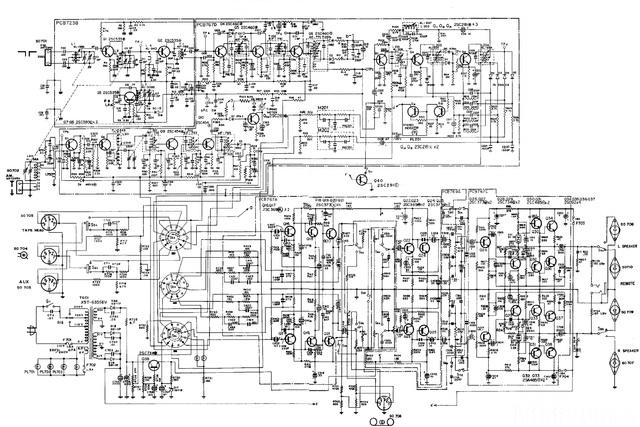
\includegraphics[width=0.80\textwidth]{pics/schaltplan_.jpg}
	\caption{Spannungsteiler basierte Ansteuerung einer LED}
	\label{fig:schaltplan}
\end{figure}
\\
\subsubsection{Verifikation}
Die Schaltung wird mit einer 0~V Quelle betrieben. .....\\
Messkurven, Foto,...
\\
\subsubsection{Auswertung}
Die LED leuchtet!!!!
\subsection{Zusammenfassung}

